\section{Montaje Físico, Soluciones DIY y Registro de Troubleshooting}

\subsection{Soluciones de Ingeniería DIY en el Ensamble Mecánico}
El diseño físico del biorreactor presentó retos mecánicos y termodinámicos sustanciales al utilizar componentes comerciales de bajo costo para alcanzar prestaciones de laboratorio. Las soluciones implementadas fueron:

\begin{enumerate}[label=\textbf{\arabic*.}]
    \item \textbf{Cuerpo del Reactor en Botella PET Transparente:}
    Se seleccionó un envase cilíndrico de PET por su alta transparencia lumínica (fundamental para la fotosíntesis de \textit{Tetraselmis chuii}), inocuidad química y facilidad de maquinado para sellos herméticos.

    \item \textbf{Sistema de Homogeneización por Burbujeo (Aireador):}
    En fluidos estacionarios, el agua se estratifica térmicamente con facilidad (el líquido frío decanta en el fondo mientras el agua tibia sube). Para resolver esto, introduje una manguera de burbujeo continuo desde la base conectada a un compresor de acuario. Esto produce dos beneficios capitales:
    \begin{itemize}
        \item Mezcla convectiva forzada continua que homogeneiza la masa líquida, garantizando que el sensor DS18B20 registre la temperatura volumétrica real.
        \item Suministro constante de intercambio gaseoso ($CO_2$ para fotosíntesis y desorción de $O_2$ disuelto).
    \end{itemize}

    \item \textbf{Acoplamiento Térmico Mecánico por Compresión (Zuncho Metálico):}
    Uno de los mayores desafíos fue acoplar una celda Peltier rígida y estrictamente plana ($40 \times 40\,\text{mm}$) contra las paredes curvas y deformables de la botella PET. Diseñé un mecanismo de sujeción basado en una abrazadera metálica de presión (zuncho de manguera) que comprime una placa de interfaz de aluminio con pasta térmica contra la pared plástica. La presión controlada deforma el PET lo justo para generar un plano de transferencia térmica íntimo y continuo sin fisurar el plástico.

    \item \textbf{Torre de Disipación de CPU de Alto Rendimiento (KF200-DGT):}
    Una celda Peltier genera en su cara caliente la suma del calor extraído más toda la potencia eléctrica consumida ($Q_h = Q_c + V \cdot I \approx 15\,\text{W} + 50\,\text{W} = 65\,\text{W}$). Para evitar que este calor se filtre de regreso a la cara fría, acoplé un disipador de torre KF200-DGT equipado con tubos de calor (\textit{heatpipes}) de cobre y ventilador de alto flujo.
\end{enumerate}

\begin{figure}[htbp]
    \centering
    \begin{subfigure}[b]{0.48\textwidth}
        \centering
        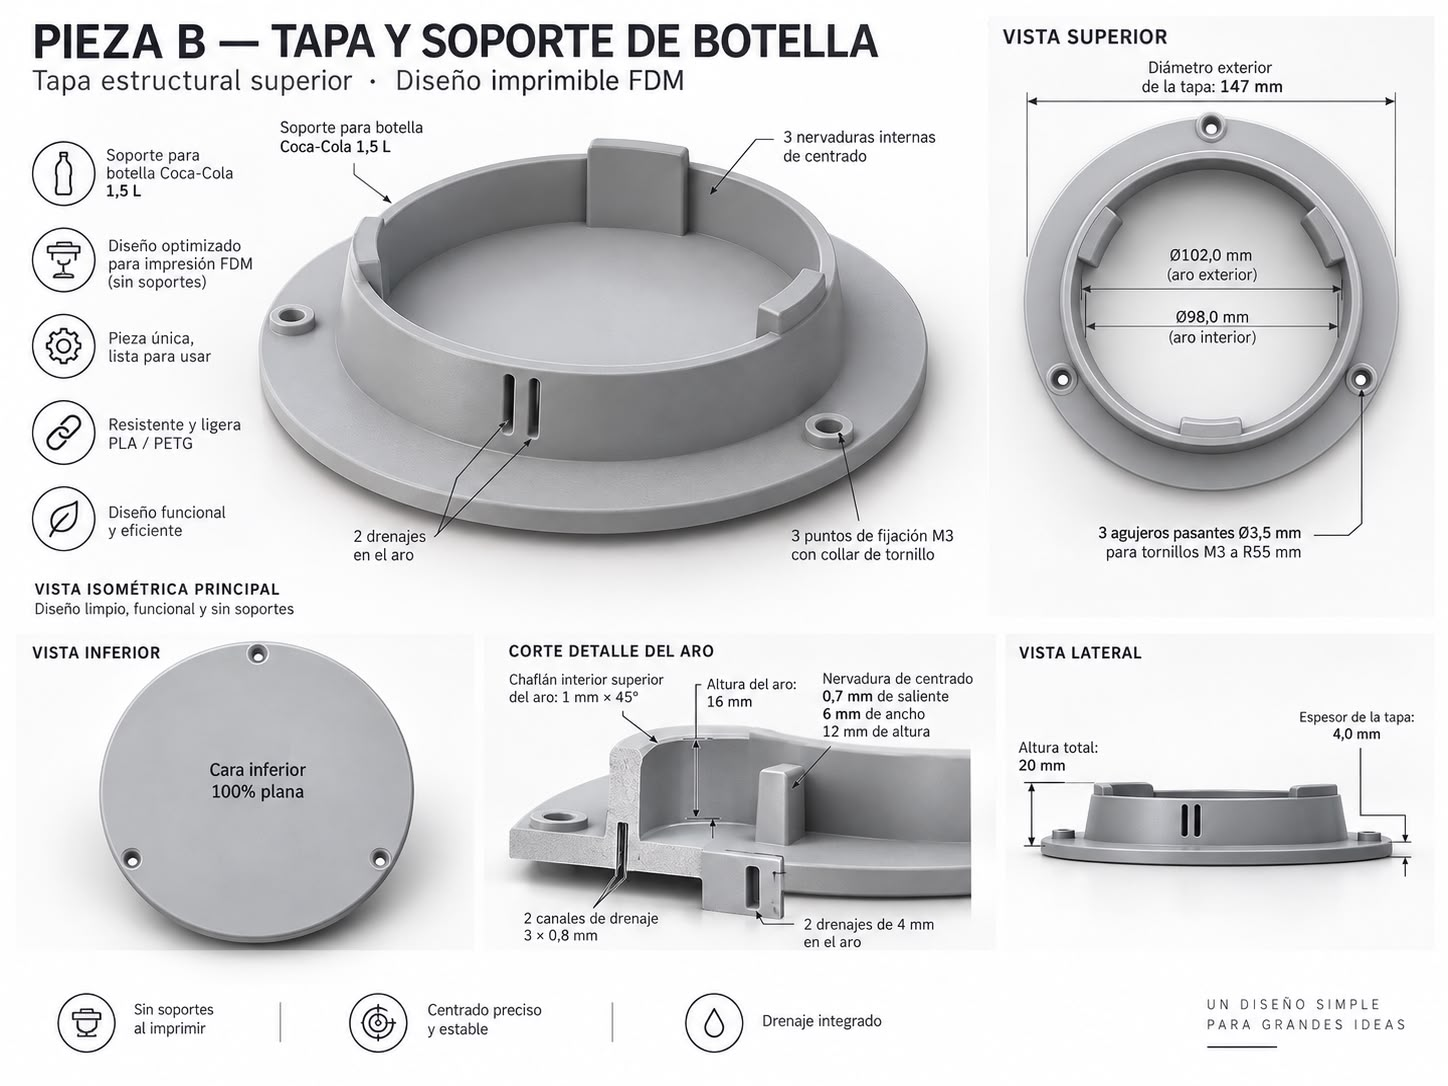
\includegraphics[width=\textwidth]{imagenes/botella_aireador.jpeg}
        \caption{Tanque PET con sensor sumergido y aireación.}
        \label{fig:tanque_pet}
    \end{subfigure}
    \hfill
    \begin{subfigure}[b]{0.48\textwidth}
        \centering
        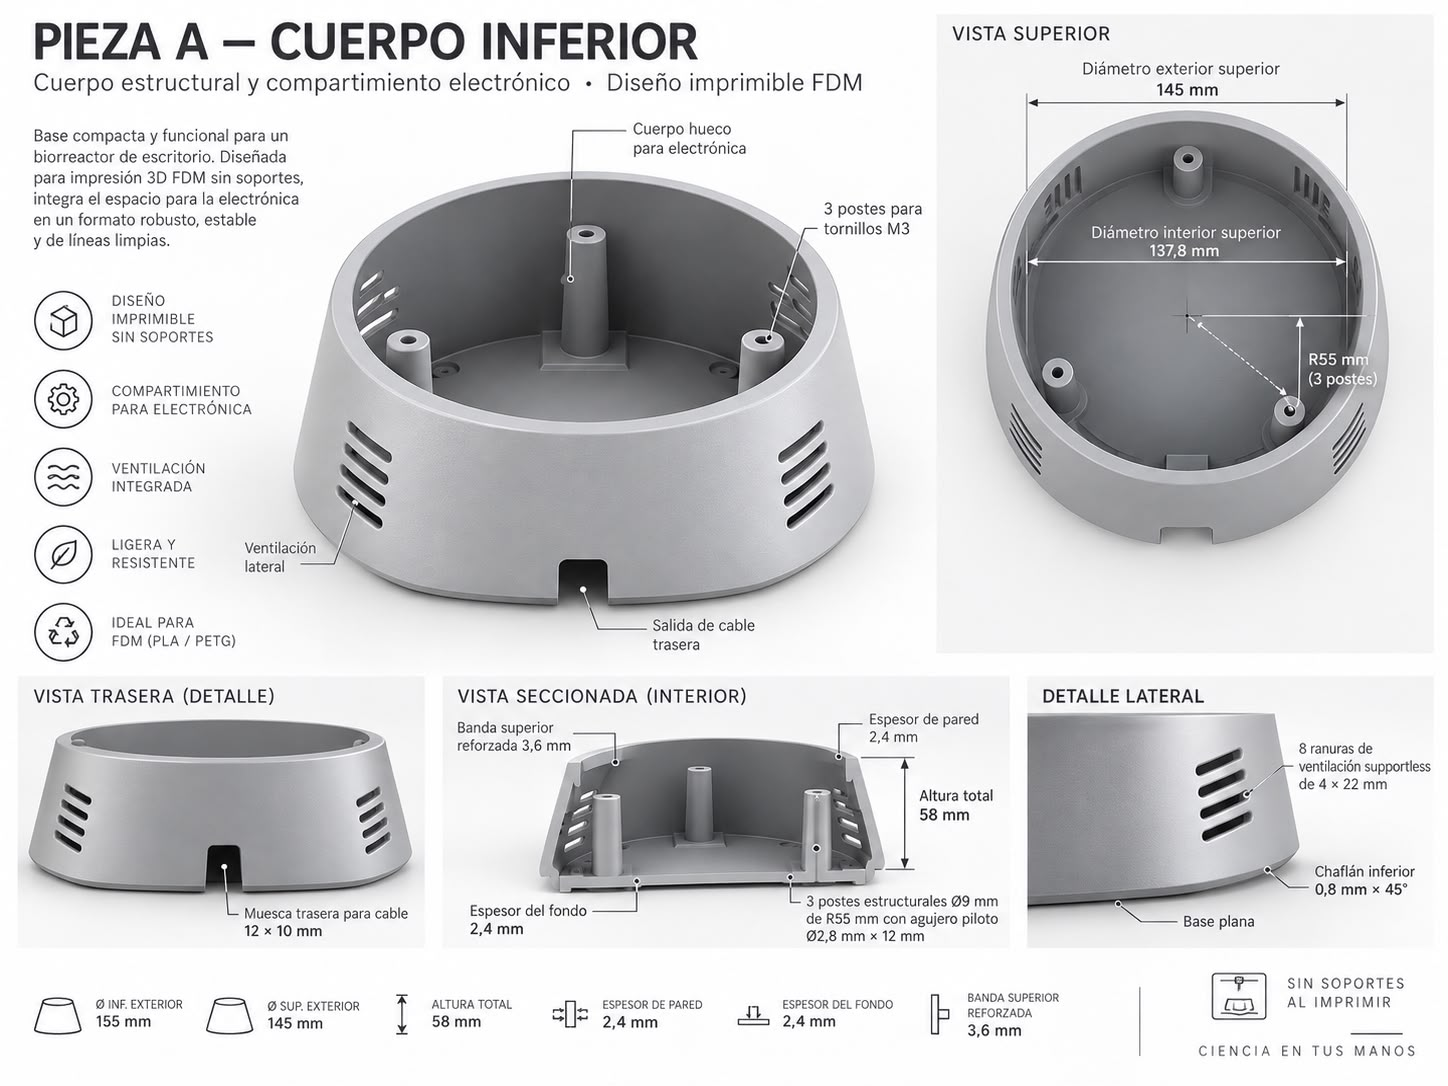
\includegraphics[width=\textwidth]{imagenes/acople_zuncho.jpeg}
        \caption{Acople mecánico de presión con zuncho metálico.}
        \label{fig:acople_zuncho}
    \end{subfigure}
    \\[0.3cm]
    \begin{subfigure}[b]{0.48\textwidth}
        \centering
        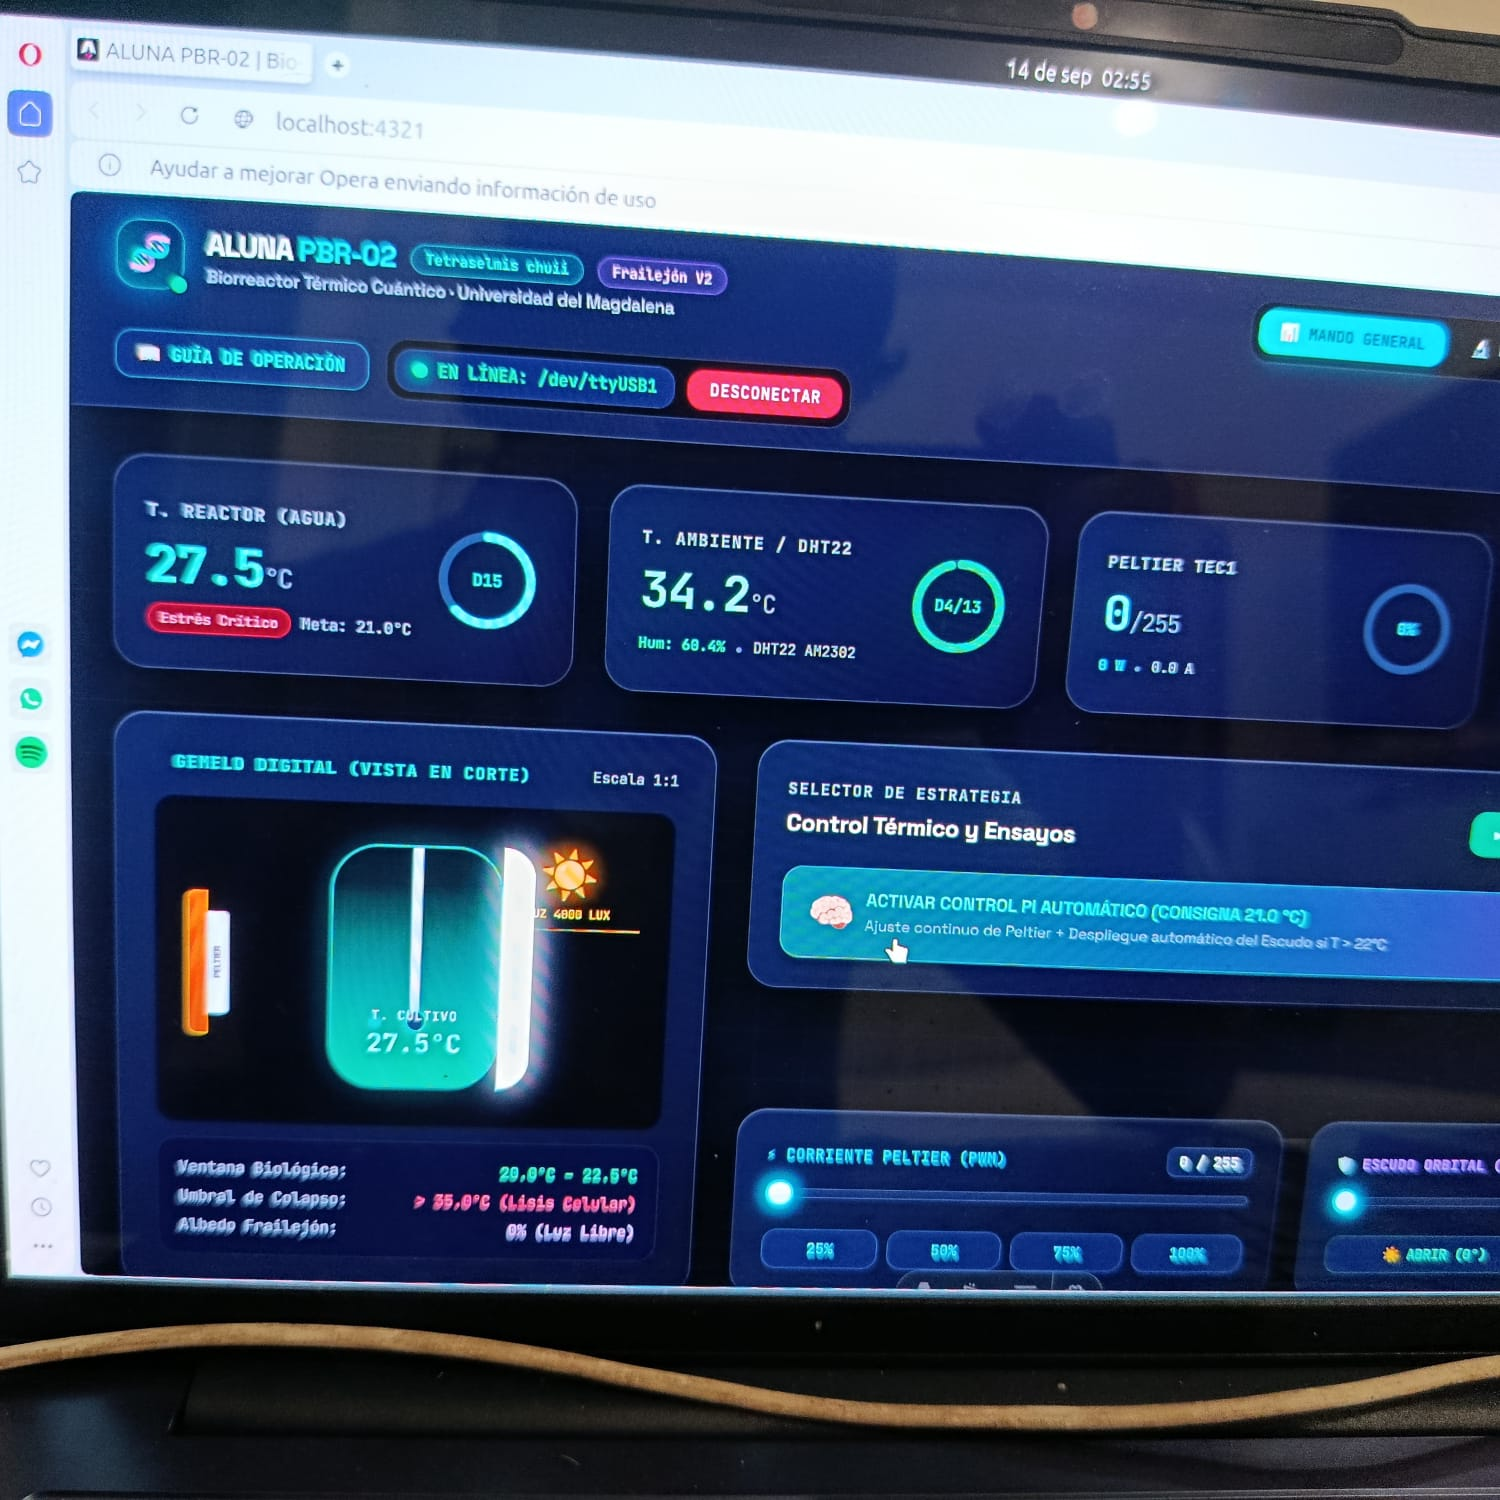
\includegraphics[width=\textwidth]{imagenes/disipador_kf200.jpeg}
        \caption{Disipador KF200-DGT con tubos de cobre.}
        \label{fig:disipador}
    \end{subfigure}
    \hfill
    \begin{subfigure}[b]{0.48\textwidth}
        \centering
        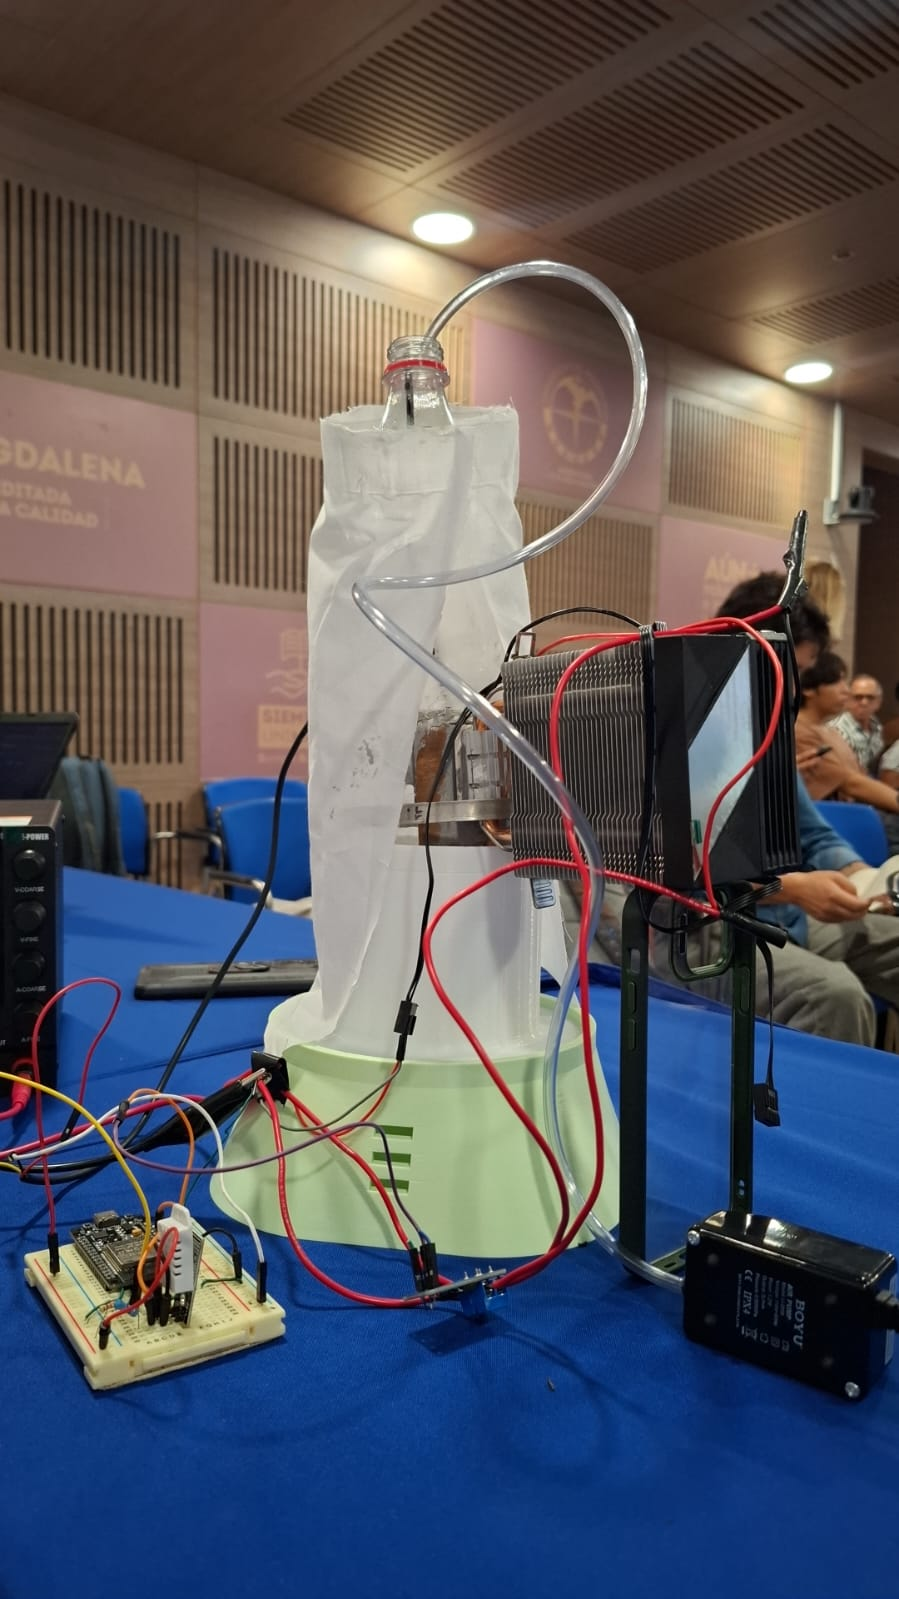
\includegraphics[width=\textwidth]{imagenes/prototipo_final.jpeg}
        \caption{Ensamble completo operando en banco.}
        \label{fig:prototipo_completo}
    \end{subfigure}
    \caption{Fotografías del proceso constructivo y ensamble final del fotobiorreactor ALUNA PBR-02.}
    \label{fig:galeria_fotos}
\end{figure}

\subsection{Registro Exhaustivo de Fallas Experimentales (Troubleshooting)}
Durante las pruebas de estrés en banco de trabajo, documenté, diagnostiqué y superé cuatro fallas críticas de ingeniería:

\subsubsection{Falla 1: Inversión de Polaridad en la Celda Termoeléctrica}
\begin{itemize}
    \item \textbf{Síntoma Observado:} Al energizar la etapa de potencia al 100\% PWM, los tubos de cobre del disipador descendieron bruscamente a temperaturas gélidas ($< 15\,^\circ\text{C}$), mientras que el agua del reactor comenzó a calentarse de forma acelerada ($> 30\,^\circ\text{C}$).
    \item \textbf{Diagnóstico Físico:} Por efecto Peltier, el sentido del flujo térmico depende exclusivamente de la dirección de la corriente continua. La polaridad en los bornes del módulo MOSFET estaba invertida, por lo que la celda bombeaba calor desde el ambiente hacia el reactor.
    \item \textbf{Solución Aplicada:} Inversión física de los terminales en las borneras \texttt{OUT+} y \texttt{OUT-} del MOSFET D4184, normalizando la extracción de calor desde el agua hacia el disipador exterior.
\end{itemize}

\subsubsection{Falla 2: Cuello de Botella Térmico por Conductividad del PET}
\begin{itemize}
    \item \textbf{Síntoma Observado:} La placa metálica de contacto alcanzaba temperaturas de escarcha ($< 2\,^\circ\text{C}$), pero la temperatura del agua descendía a una tasa muy lenta ($\approx 0.05\,^\circ\text{C/min}$).
    \item \textbf{Diagnóstico Físico:} El tereftalato de polietileno (PET) es un pésimo conductor térmico ($k_{\text{PET}} \approx 0.15 - 0.24\,\text{W/(m}\cdot\text{K)}$ frente a $k_{\text{Al}} \approx 205\,\text{W/(m}\cdot\text{K)}$ del aluminio). Además, las paredes expuestas de la botella absorbían continuamente calor por convección del ambiente cálido de Santa Marta ($32\,^\circ\text{C}$).
    \item \textbf{Solución y Ajuste:} Se aumentó la presión del zuncho para adelgazar la película plástica en el punto de contacto, se garantizó pasta térmica siliconada de alta densidad y se diseñó la adición de una camisa perimetral aislante de espuma elastomérica.
\end{itemize}

\subsubsection{Falla 3: Pérdida de Tensión y Limitación de Corriente por Resistencia de Contacto}
\begin{itemize}
    \item \textbf{Síntoma Observado:} Con la fuente fijada en $12.0\,\text{V}$, la celda Peltier consumía únicamente $1.8\,\text{A}$ en lugar de los $4.0\,\text{A}$ esperados según su hoja de datos.
    \item \textbf{Diagnóstico Eléctrico:} Concurrencia de dos fenómenos:
    \begin{enumerate}
        \item Los cables de prototipo (tipo Dupont) introducían una resistencia parásita no despreciable en serie ($R_{\text{cable}} \approx 0.5\,\Omega$).
        \item La tensión de compuerta $V_{GS} = 3.3\,\text{V}$ entregada por la ESP32 no saturaba completamente los canales de los transistores D4184 (que requieren $V_{GS} \ge 4.5\,\text{V}$ para $R_{DS(\text{on})}$ mínima).
        \item El Efecto Seebeck inverso genera una fuerza contraelectromotriz ($V_{\text{fem}} = \alpha_{te} \Delta T$) que se opone a la fuente a medida que la celda se enfría.
    \end{enumerate}
    \item \textbf{Solución Aplicada:} Sustitución del cableado de potencia por conductores de cobre de calibre AWG 18 soldados directamente, y ajuste de la tensión de la fuente de poder a $13.5\,\text{V}$, restaurando el consumo nominal en $3.8 - 4.1\,\text{A}$.
\end{itemize}

\subsubsection{Falla 4: Desincronización de Telemetría en el Dashboard Web}
\begin{itemize}
    \item \textbf{Síntoma Observado:} El servidor backend recibía tramas seriales válidas de la ESP32, pero las gráficas de ECharts en el navegador no se actualizaban y la consola arrojaba un error \texttt{ReferenceError: latest is not defined}.
    \item \textbf{Diagnóstico de Software:} La estructura de datos del endpoint REST fue refactorizada en el servidor para añadir campos, pero el frontend aún procesaba el formato anterior. Asimismo, desconexiones breves en el bus 1-Wire inyectaban valores nulos que interrumpían la gráfica.
    \item \textbf{Solución Aplicada:} Estandarización estricta del esquema JSON, corrección del mapeo en Astro y filtrado de lecturas espurias de bus abierto (como $-127.0\,^\circ\text{C}$ o $+85.0\,^\circ\text{C}$).
\end{itemize}
